\documentclass[a4paper]{article}

\usepackage[utf8]{inputenc}
\usepackage[T1]{fontenc}
\usepackage{textcomp}
\usepackage[english]{babel}
\usepackage{amsmath, amssymb}


%figure support
\usepackage{import}
\usepackage{xifthen}
\pdfminorversion=7
\usepackage{pdfpages}
\usepackage{transparent}
\newcommand{\incfig}[1]{%
	\def\svgwidth{\columnwidth}
	\import{./figures/}{#1.pdf_tex}
}
\graphicspath{ {./figures/} }
\pdfsuppresswarningpagegroup=1

\begin{document}
	\title{CAP 4630.01 Assignment 6 Due 11/13/19}
	\author{Brandon Thompson 5517}
	\maketitle

	Given the following Bayesian belief network and probability tables, please figure
	out the joint probability of:
	\begin{equation*}
		P\left( A \cap \overline{B} \cap \overline{C} \cap D \right) 
	\end{equation*}
	\begin{figure}[ht!]
		\centering
		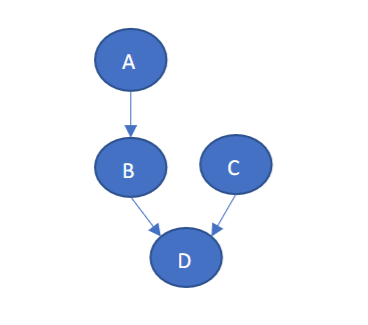
\includegraphics[width=0.4\textwidth]{assignment6_fig}
		\caption{Bayesian Belief network}
		\label{fig:1}
	\end{figure}

	\begin{center}
		\begin{tabular}{| c |}
			\hline
			$P\left( A \right) $ \\
			\hline
			$a\%$ \\
			\hline
		\end{tabular}
	\end{center}

	\begin{center}
		\begin{tabular}{| c | c |}
			\hline
			{$A$ & $P\left( B \right) $ \\
			\hline
			true & $b\%$ \\
			\hline
			false & $c\%$ \\
			\hline
		\end{tabular}
	\end{center}

	\begin{center}
		\begin{tabular}{| c |}
			\hline
			$P\left( C \right) $\\
			\hline
			$d\%$ \\
			\hline
		\end{tabular}
	\end{center}

	\begin{center}
		\begin{tabular}{| c | c | c |}
			\hline
			$B$ & $C$ & $P\left( D \right) $ \\
			\hline
			true & true & $e\%$ \\
			\hline
			true & false & $f\%$ \\
			\hline
			false & true & $g\%$ \\
			\hline
			false & false & $h\%$ \\
			\hline
		\end{tabular}
	\end{center}
\clearpage
	\begin{align*}
		P(\overline{C}) &= 1-d\%\\
		P(\overline{B}|A) &= 1-b\%
	\end{align*}

\begin{equation*}	
	\begin{split}
		P(A \cap \overline{B} \cap \overline{C} \cap D )& = P(A) \times P(\overline{B}| A) \times P(\overline{C}) \times P(D|B \cap C)\\
		& = a\% \times (1-b\%) \times (1-d\%) \times e\%
	\end{split}
\end{equation*}
\end{document}
